%%%%%%%%%%%%%%%%%%%%%%%%%%%%%%%%%%%%%%%%%
% Journal Article
% Data Structures and Algorithm
% Practical 1: Analyze running complexity of various sorting algorithm
%
% Gahan M. Saraiya
% 18MCEC10
%
%%%%%%%%%%%%%%%%%%%%%%%%%%%%%%%%%%%%%%%%%
%----------------------------------------------------------------------------------------
%       PACKAGES AND OTHER DOCUMENT CONFIGURATIONS
%----------------------------------------------------------------------------------------
\documentclass[paper=letter, fontsize=12pt]{article}
\usepackage[english]{babel} % English language/hyphenation
\usepackage{amsmath,amsfonts,amsthm} % Math packages
\usepackage[utf8]{inputenc}
\usepackage{float}
\usepackage{lipsum} % Package to generate dummy text throughout this template
\usepackage{blindtext}
\usepackage{graphicx} 
\usepackage{caption}
\usepackage{subcaption}
\usepackage[sc]{mathpazo} % Use the Palatino font
\usepackage[T1]{fontenc} % Use 8-bit encoding that has 256 glyphs
\usepackage{bbding}  % to use custom itemize font
\linespread{1.05} % Line spacing - Palatino needs more space between lines
\usepackage{microtype} % Slightly tweak font spacing for aesthetics
\usepackage[hmarginratio=1:1,top=32mm,columnsep=20pt]{geometry} % Document margins
\usepackage{multicol} % Used for the two-column layout of the document
%\usepackage[hang, small,labelfont=bf,up,textfont=it,up]{caption} % Custom captions under/above floats in tables or figures
\usepackage{booktabs} % Horizontal rules in tables
\usepackage{float} % Required for tables and figures in the multi-column environment - they need to be placed in specific locations with the [H] (e.g. \begin{table}[H])
\usepackage{hyperref} % For hyperlinks in the PDF
\usepackage{lettrine} % The lettrine is the first enlarged letter at the beginning of the text
\usepackage{paralist} % Used for the compactitem environment which makes bullet points with less space between them
\usepackage{abstract} % Allows abstract customization
\renewcommand{\abstractnamefont}{\normalfont\bfseries} % Set the "Abstract" text to bold
\renewcommand{\abstracttextfont}{\normalfont\small\itshape} % Set the abstract itself to small italic text
\usepackage{titlesec} % Allows customization of titles

\renewcommand\thesection{\Roman{section}} % Roman numerals for the sections
\renewcommand\thesubsection{\Roman{subsection}} % Roman numerals for subsections

\titleformat{\section}[block]{\large\scshape\centering}{\thesection.}{1em}{} % Change the look of the section titles
\titleformat{\subsection}[block]{\large}{\thesubsection.}{1em}{} % Change the look of the section titles
\newcommand{\horrule}[1]{\rule{\linewidth}{#1}} % Create horizontal rule command with 1 argument of height
\usepackage{fancyhdr} % Headers and footers
\pagestyle{fancy} % All pages have headers and footers
\fancyhead{} % Blank out the default header
\fancyfoot{} % Blank out the default footer


%----------------------------------------------------------------------------------------
%----------------------------------------------------------------------------------------
%       CUSTOM HEADER TEXT
%----------------------------------------------------------------------------------------
\fancyhead[C]{Institute of Technology, Nirma University $\bullet$ 25 September 2018} % Custom header text
%----------------------------------------------------------------------------------------

\fancyfoot[RO,LE]{\thepage} % Custom footer text
%----------------------------------------------------------------------------------------
%       PACKAGE for code highlight
%----------------------------------------------------------------------------------------
\usepackage[utf8]{inputenc}
\usepackage[english]{babel}

\usepackage{minted} % for highlighting code sytax
%----------------------------------------------------------------------------------------
%       TITLE SECTION
%----------------------------------------------------------------------------------------
\title{\vspace{-15mm}\fontsize{24pt}{10pt}\selectfont\textbf{
		\underline{Practical 1}\\Analyze running complexity of various sorting algorithm}} % Article title
\author{\large{\textsc{
		Gahan M. Saraiya, 18MCEC10 }}\\[2mm]
%\thanks{A thank you or further information}\\ % Your name
\normalsize \href{mailto:18mcec10@nirmauni.ac.in}{18mcec10@nirmauni.ac.in}\\[2mm] % Your email address
}
\date{}
\hypersetup{
	colorlinks=true,
	linkcolor=blue,
	filecolor=magenta,      
	urlcolor=cyan,
	pdfauthor={Gahan M. Saraiya},
	pdfcreator={Gahan M. Saraiya},
	pdfproducer={Gahan M. Saraiya},
}
%----------------------------------------------------------------------------------------

\begin{document}
\maketitle % Insert title
\thispagestyle{fancy} % All pages have headers and footers

\newcommand*\tick{\item[\Checkmark]}
\newcommand*\arrow{\item[$\Rightarrow$]}
\newcommand*\fail{\item[\XSolidBrush]}

\section{Introduction}
\paragraph{}
Aim of this practical is to analyze the time complexity of sorting algorithms for various input size.

\textbf{Algorithms} analyzed are listed below:
\begin{itemize}
	\item Bubble Sort
	\item Insertion Sort
	\item Selection Sort
	\item Quick Sort
	\item Merge Sort
	\item Heap Sort
\end{itemize}

\section{Implementation}

\subsection{Utility \textbf{\textit{utility.h}}}
\inputminted[frame=lines, breaklines, linenos]{c}{../utility.h}

\subsection{Constants \textbf{\textit{constant.h}}}
\inputminted[frame=lines, breaklines, linenos]{c}{../constant.h}

\subsection{Sorting Algorithms \textbf{\textit{sorting\_algorithms.h}}}
\inputminted[frame=lines, breaklines, linenos]{c}{../sorting_algorithms.h}


\subsection{Main Program - \textbf{\textit{program.c}}}
\inputminted[frame=lines, breaklines, linenos]{c}{../program.c}

\section{Analysis}
All mentioned algorithms are tested for input length: $ 10 $, $ 10^1 $, $ 10^2 $, $ 10^3 $, $ 10^4 $, $ 10^5 $
with various array construction listed below:
\begin{itemize}
	\item All elements are in ascending order
	\item All elements are in descending order
	\item All elements are in random order
	\item All elements are same
\end{itemize}
\subsection{Bubble Sort}
\begin{figure}[H]
	\centering
	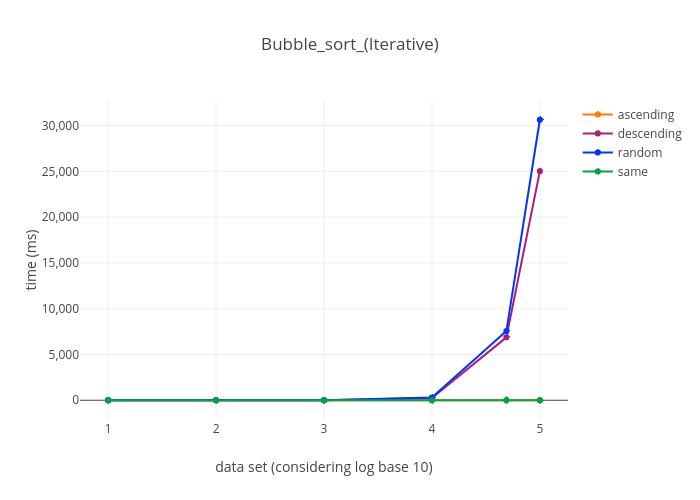
\includegraphics[scale=0.75]{../analysis/Bubble_sort_(Iterative).png}
	\caption{Bubble Sort}
\end{figure}

\subsection{Insertion Sort}
\begin{figure}[H]
	\centering
	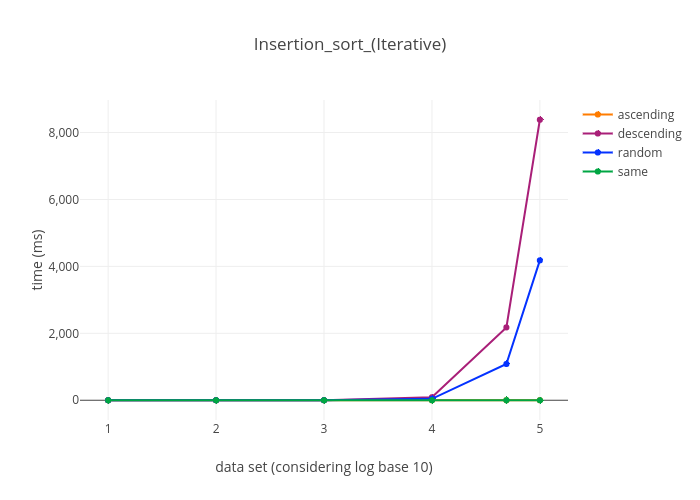
\includegraphics[scale=0.75]{../analysis/Insertion_sort_(Iterative).png}
	\caption{Insertion Sort}
\end{figure}

\subsection{Selection Sort}
\begin{figure}[H]
	\centering
	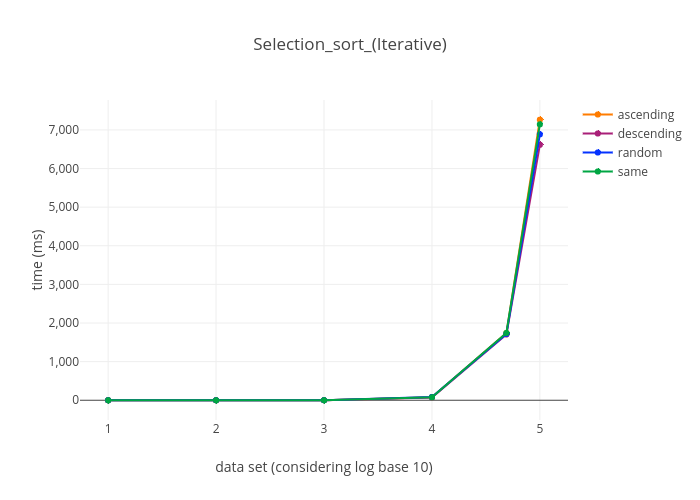
\includegraphics[scale=0.75]{../analysis/Selection_sort_(Iterative).png}
	\caption{Selection Sort}
\end{figure}

\subsection{Quick Sort}
\begin{figure}[H]
	\centering
	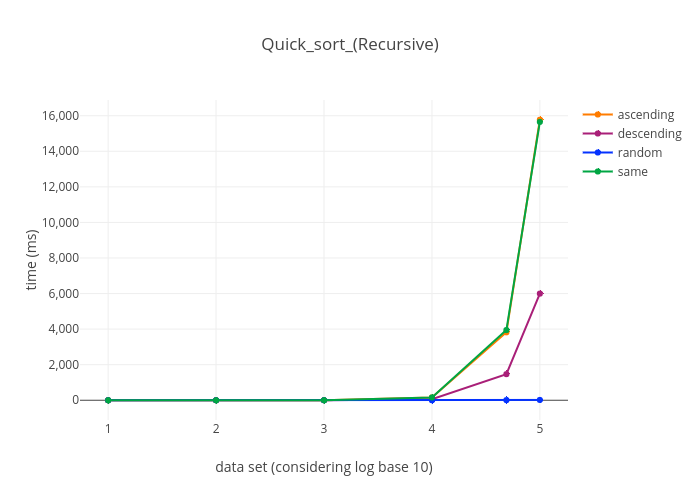
\includegraphics[scale=0.75]{../analysis/Quick_sort_(Recursive).png}
	\caption{Quick Sort}
\end{figure}

\subsection{Merge Sort}
\begin{figure}[H]
	\centering
	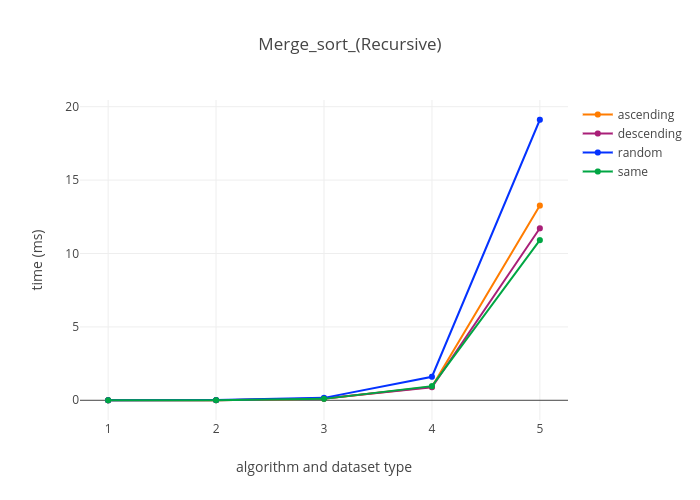
\includegraphics[scale=0.75]{../analysis/Merge_sort_(Recursive).png}
	\caption{Merge Sort}
\end{figure}

\subsection{Heap Sort}
\begin{figure}[H]
	\centering
	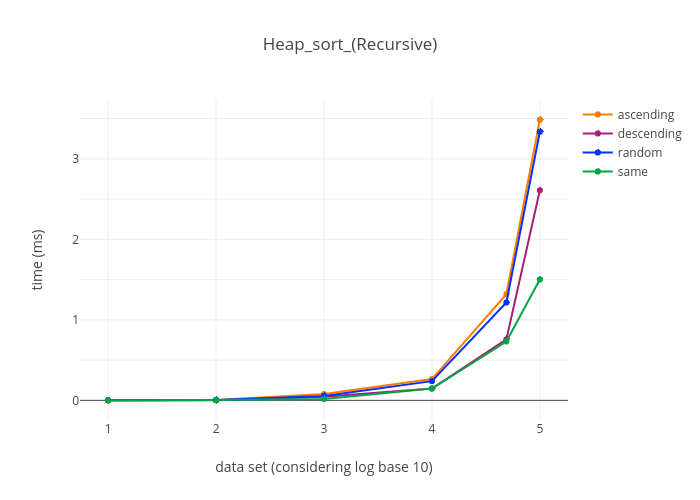
\includegraphics[scale=0.75]{../analysis/Heap_sort_(Recursive).png}
	\caption{Heap Sort}
\end{figure}
%
%\section*{Output 2}
%\inputminted[frame=lines, breaklines]{text}{output2.txt}
%
%\section*{Output 3}
%\inputminted[frame=lines, breaklines]{text}{output3.txt}

\section{Summary}
\begin{itemize}
	\tick If directory fits in memory then point query requires only $ 1 $ disk access
	\tick Empty buckets can be merge with it's split image when directory becomes half of size
\end{itemize}
%----------------------------------------------------------------------------------------
%\end{multicols}
\end{document}
